% c:\Cursos\Udemy\Desenvolvimento Web Completo\Web-Projects\APS\relatorio.tex
\documentclass[12pt,a4paper]{article}
\usepackage[portuguese]{babel}
\usepackage[utf8]{inputenc}
\usepackage{geometry}
\usepackage{setspace}
\usepackage{hyperref}
\usepackage{tocloft}
\usepackage{graphicx}
\usepackage{float}
\geometry{left=3cm,right=2cm,top=3cm,bottom=2cm}
\setlength{\parindent}{1.25cm}
\setlength{\parskip}{0.2cm}
\onehalfspacing

\begin{document}

% Capa
\begin{titlepage}
    \begin{center}
        \vspace*{2.5cm}
        \textbf{UNIVERSIDADE POSITIVO}\\[0.8cm]
        \textbf{ANÁLISE E DESENVOLVIMENTO DE SISTEMAS}\\[3cm]
        \textbf{Documentação Final}\\[3cm]
        Alunos:\\[0.5cm]
        Marcelo Nassar de Souza da Silva\\[0.3cm]
        Matheus Alves de Lima\\[0.3cm]
        Luigi Roehrig Segala
        \vfill
        Curitiba\\[0.2cm]
        06/2025
    \end{center}
\end{titlepage}
\newpage

% Sumário
\tableofcontents
\newpage

\section{Introdução}
Este documento descreve o projeto de desenvolvimento de uma página única (Single Page Application - SPA) para o cliente Gabriel Munhoz, fã do Paraná Clube e do jogador Cristiano Ronaldo (CR7). O site tem como objetivo apresentar informações pessoais do cliente, a história do Paraná Clube, jogadores favoritos e um jogo marcante (Paraná x Internacional em 2017).

\section{Cronograma Preliminar}
\begin{table}[h!]
\centering
\resizebox{\textwidth}{!}{%
\begin{tabular}{|l|l|l|}
\hline
\textbf{Fase} & \textbf{Período} & \textbf{Marco} \\
\hline
Início e Conhecimento & 27/03 a 09/04/2025 & Documento de especificação inicial e plano do projeto aprovados. \\
\hline
Alinhamento & 10/04 a 16/04/2025 & Requisitos finais e sitemap aprovados pelo cliente. \\
\hline
Desenvolvimento & 17/04 a 28/05/2025 & Versão beta da página com conteúdo principal implementado. \\
\hline
Testes Finais e Ajustes & 29/05 a 04/06/2025 & Página final aprovada pelo cliente. \\
\hline
Implantação & 05/06 a 11/06/2025 & Página online e entregue. \\
\hline
\end{tabular}
}
\end{table}

\section{Requisitos do Cliente}
\begin{itemize}
    \item RF01: Exibir introdução sobre Gabriel Munhoz e seus gostos pessoais.
    \item RF02: Apresentar a história do Paraná Clube.
    \item RF03: Exibir vídeo com melhores momentos do jogo Paraná x Internacional (2017).
    \item RF04: Descrever textualmente o jogo marcante.
    \item RF05: Disponibilizar informações sobre o jogador Marcão (goleiro).
    \item RF06: Disponibilizar informações sobre Cristiano Ronaldo (CR7).
    \item RF07: Permitir navegação fluida entre seções (scroll ou âncoras).
    \item RF08: Incluir cabeçalho fixo com menu de navegação.
\end{itemize}

\section{Requisitos Não-Funcionais}
\begin{itemize}
    \item Cores predominantes do Paraná Clube (vermelho, azul e branco).
    \item Design responsivo (mobile e desktop).
    \item Tempo de carregamento máximo de 3 segundos.
    \item Acesso sem autenticação.
    \item Layout simples e de fácil navegação.
\end{itemize}

\section{Restrições do Projeto}
\begin{itemize}
    \item Prazo: 27/03 a 11/06/2025.
    \item Custo: Projeto voluntário (sem custos).
    \item Tecnologias: Ferramentas gratuitas e de baixa complexidade.
    \item Equipe: 5 alunos desenvolvedores.
\end{itemize}

\section{Diagramas e Modelos}
\subsection{Modelo Esquemático dos Processos}
O modelo esquemático a seguir ilustra os principais processos do projeto, destacando o fluxo de atividades e suas inter-relações.

\begin{figure}[h!]
    \centering
    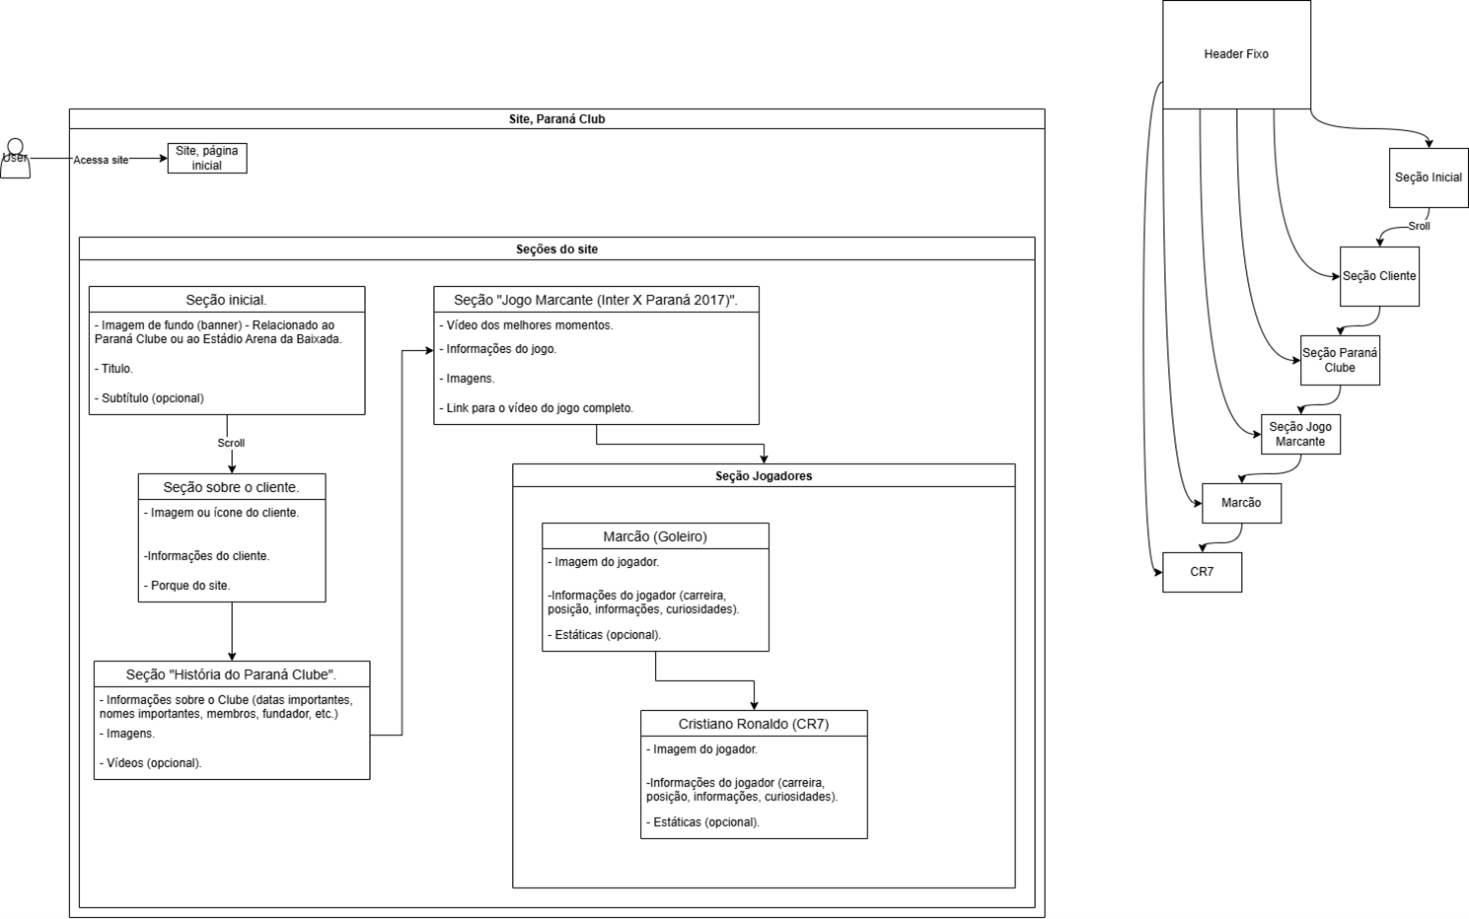
\includegraphics[width=0.9\textwidth]{modelo.png}
    \caption{Modelo esquemático dos processos do projeto}
\end{figure}

\subsection{Diagrama de Classes}
\begin{figure}[H]
   \centering
   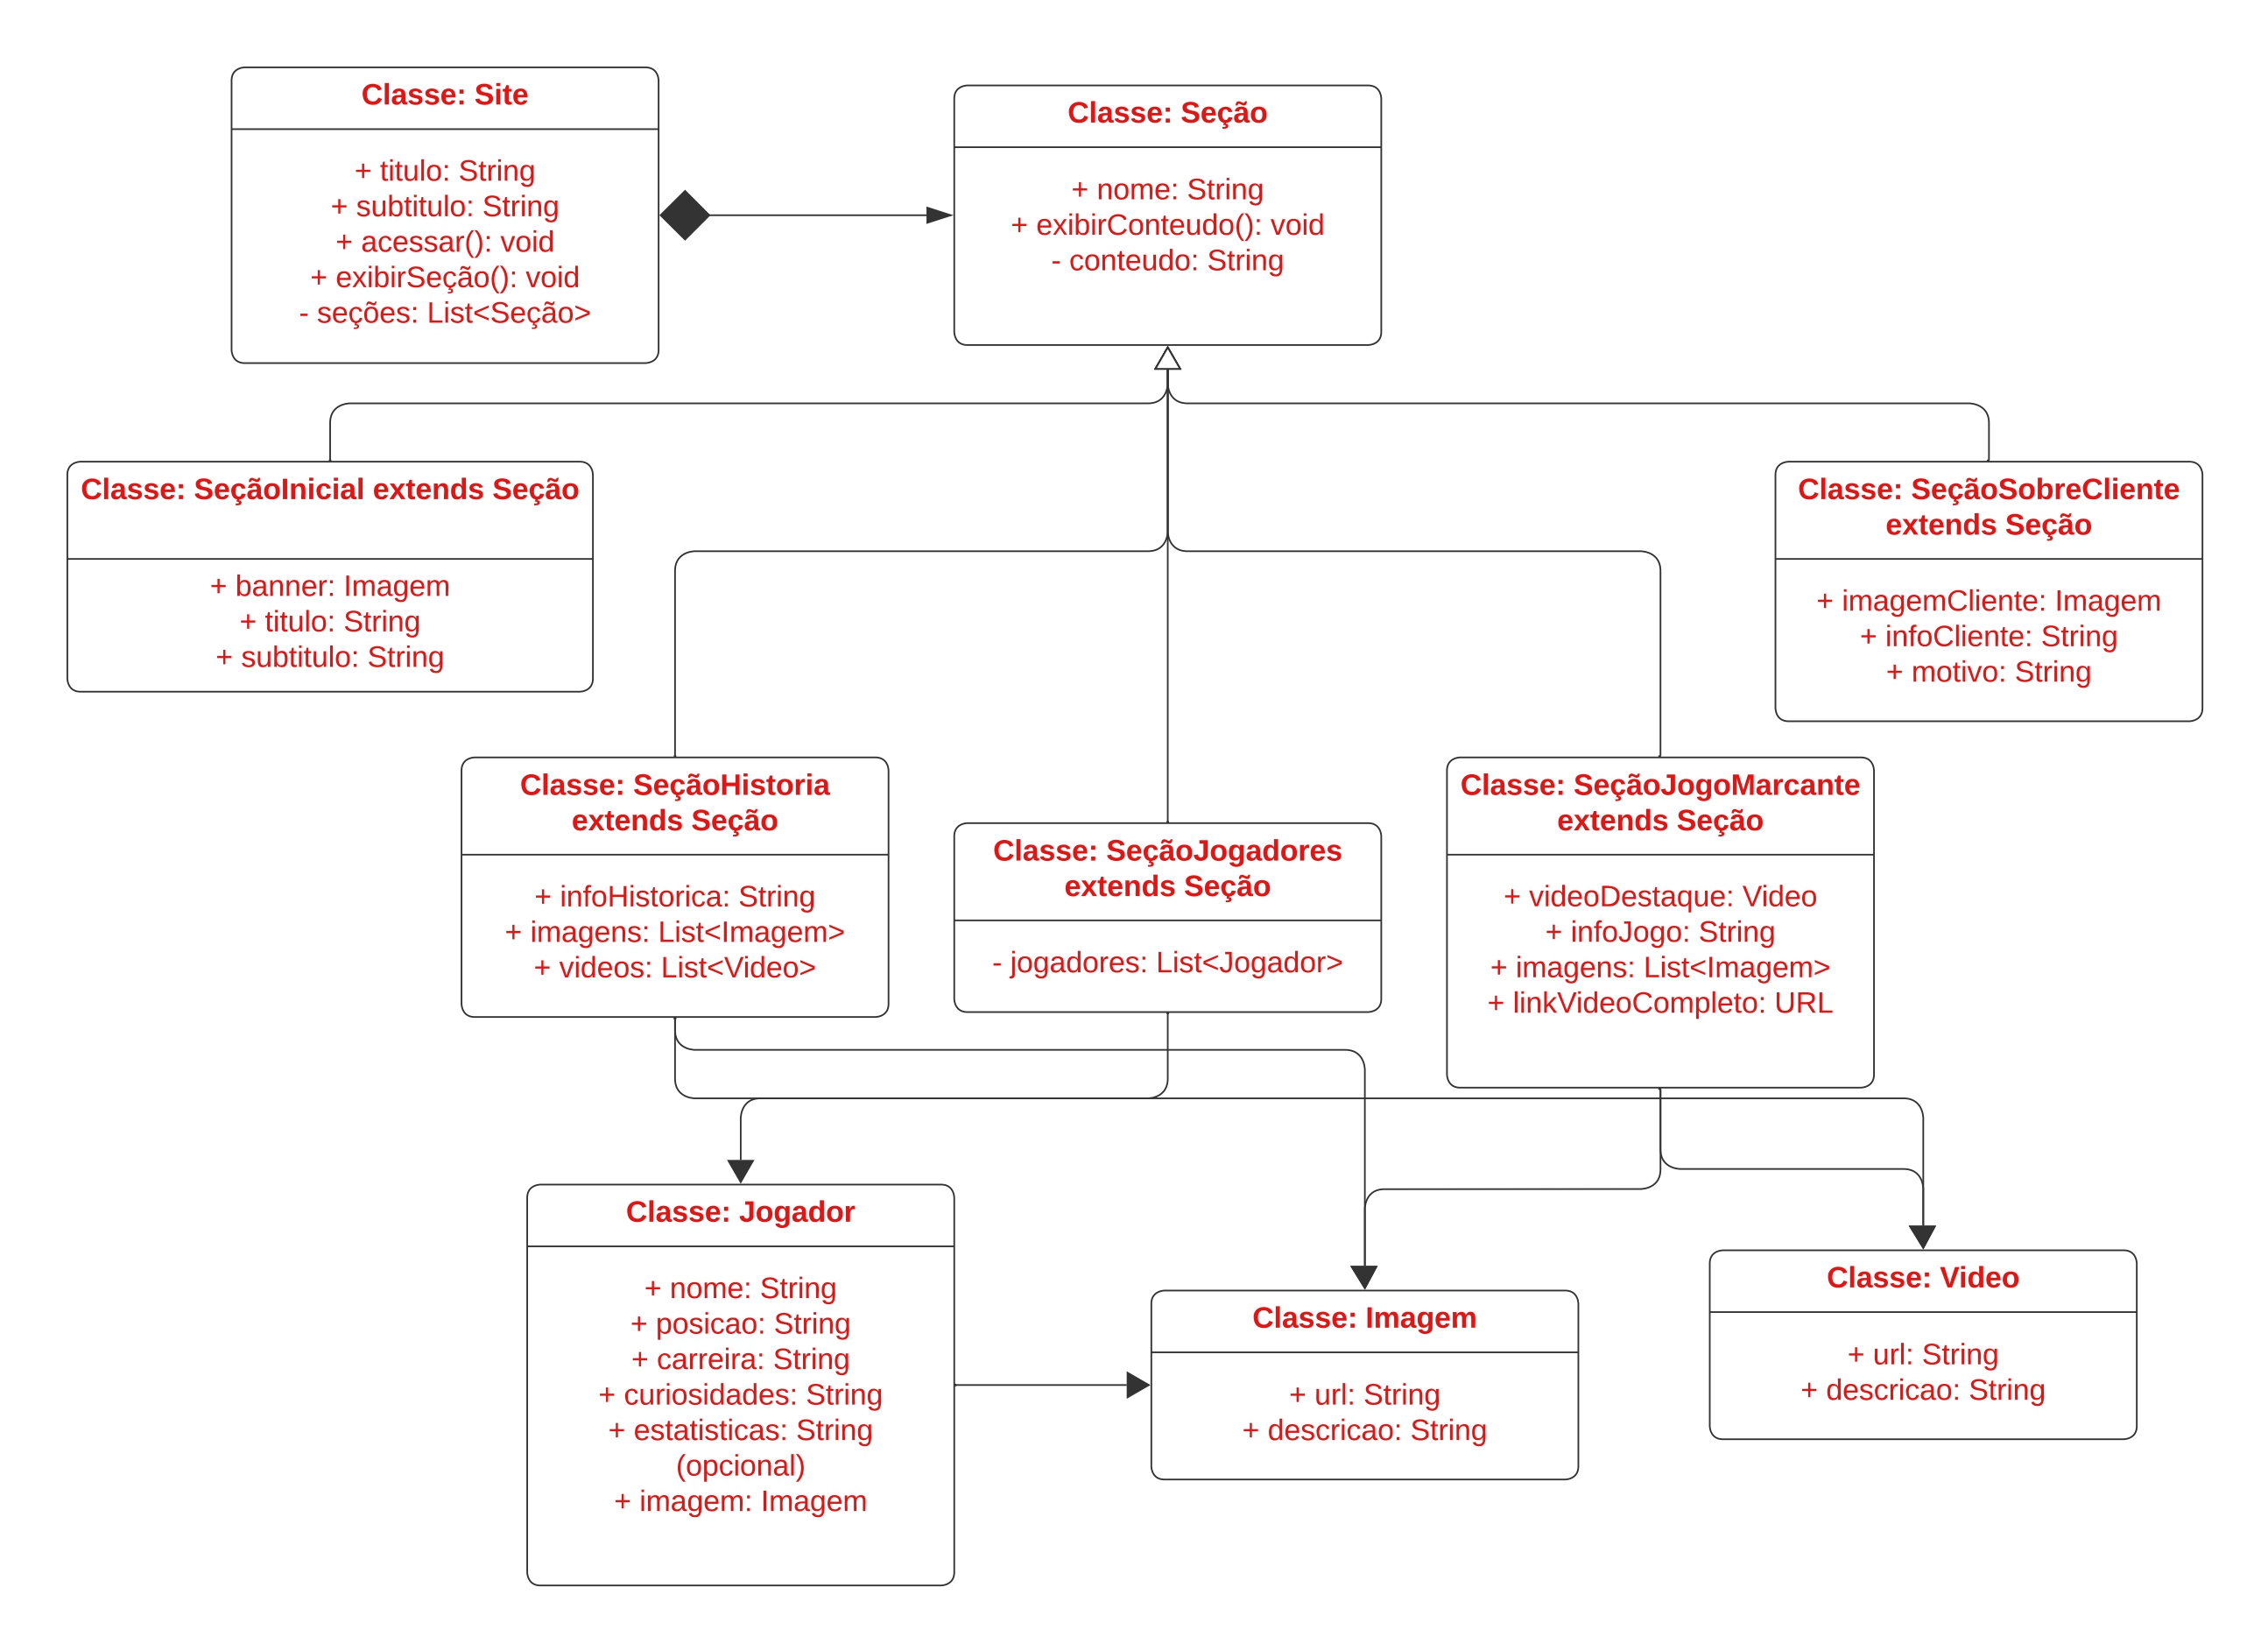
\includegraphics[width=0.8\textwidth]{Classes.jpg}
   \caption{Diagrama de Classes}
\end{figure}

\subsection{Casos de Uso}
\begin{figure}[H]
    \centering
    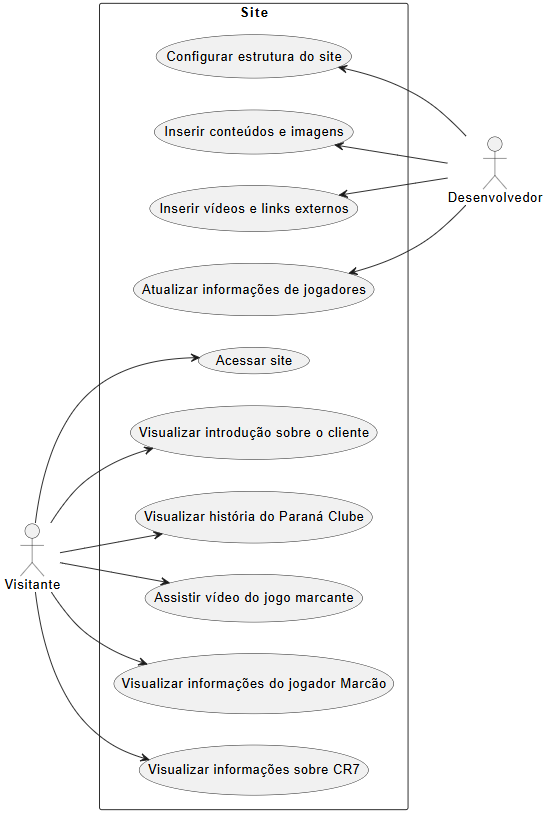
\includegraphics[width=0.9\textwidth]{casouso.png}
    \caption{Diagrama de Casos de Uso}
\end{figure}

\subsection{Diagrama de Sequência}
\begin{figure}[H]
    \centering
    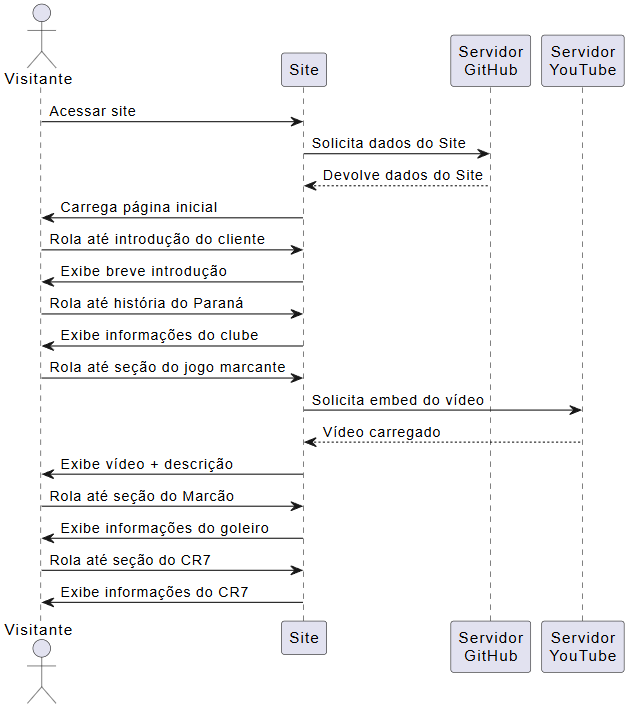
\includegraphics[width=0.9\textwidth]{sequencia.png}
    \caption{Diagrama de Sequência}
\end{figure}

\section{Matriz QFD (Quality Function Deployment)}
\begin{figure}[H]
    \centering
    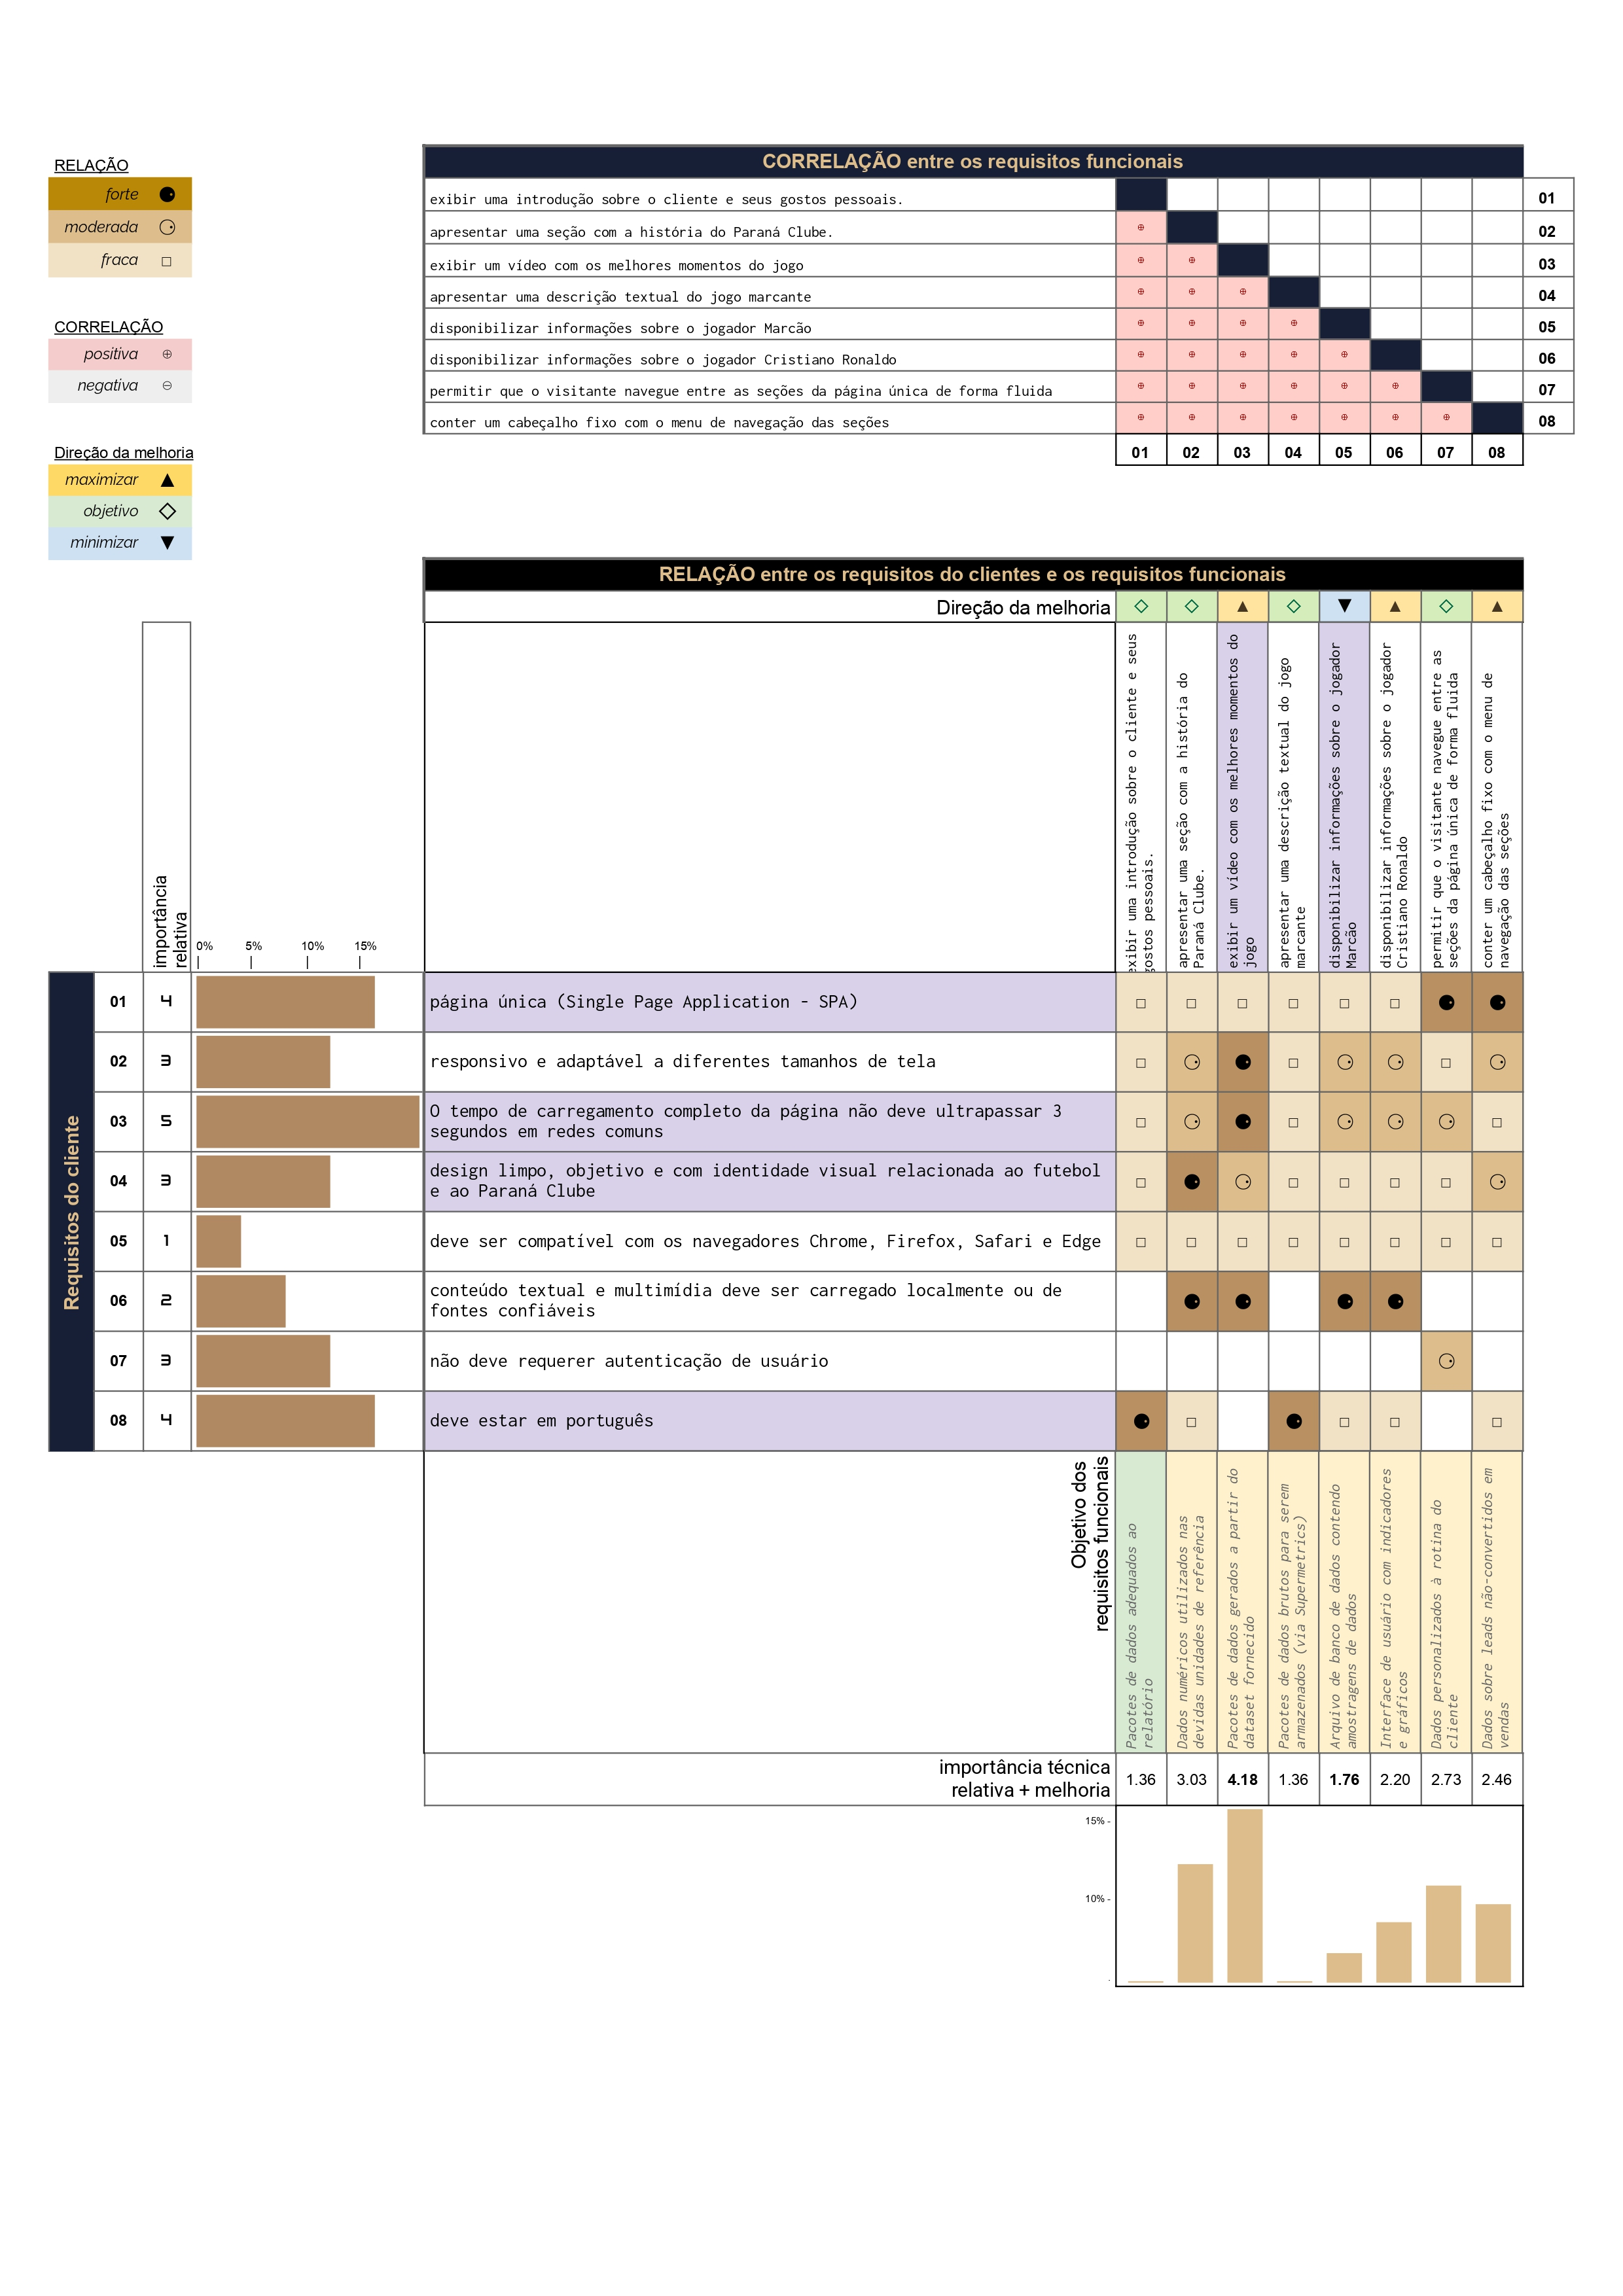
\includegraphics[width=0.9\textwidth]{matrix-qfd.jpg}
    \caption{Matriz QFD}
\end{figure}

\section{Links Relevantes}
\begin{itemize}
    \item \href{https://luigi-rs.github.io/Web-Projects/APS/}{Página Pessoal do Cliente}
    \item \href{https://github.com/Luigi-RS/Web-Projects/tree/main/APS}{Pasta do GitHub}
\end{itemize}

\section{Conclusão}
O projeto visa entregar uma página única, responsiva e alinhada aos gostos do cliente, utilizando tecnologias acessíveis e cumprindo os prazos estabelecidos. A equipe trabalhará de forma colaborativa para garantir qualidade e aderência aos requisitos.

\end{document}